\section{Context, stakeholders, expectations and scope}
\subsection{Context}
In restaurant business, the POS systems include many services such as table reservation, food ordering, alerts, billing (credit card or cash), catalogue system and processing user database
During the COVID-19 pandemic, the need of using POS systems raised dramatically because of its portability, business intelligence and reducing wasted effort and opportunity to scale a large business
Moreover, it can be easily extended for further scale of the business.

\subsection{Stakeholders}
\textbf{Managers} --- Either the restaurant owners managing the restaurant themselves or hired managers
The requirements provided by them will be directly delivered to the developers
They can provide about the feature or the UI they want to use when managing their employees.

\textbf{Clerks} --- The environment for clerks should be professional for them to deliver the convenience and time-efficiency to the customers, which is important
They should be able to tell the developers what is comfortable to use and does not waste too much time.

\textbf{Customers} --- Despite not working directly with developers, they can still contribute to the development of the software
The software will gather information from customers (with their permission) to improve the experience
Feedback features and occasional surveys will also be included to help even further.

\subsection{Expectation}
For optimizing the workflow of the restaurant and its service quality, there should be an intermediate and automated worker to handle repetitive tasks with time-efficiency and high precision
This software is expected to be a web-based Point of sale (POS) system that solves the fore-mentioned problem and it follows the business flow as described in Figure 1.

\begin{figure}[H]
  \centering
  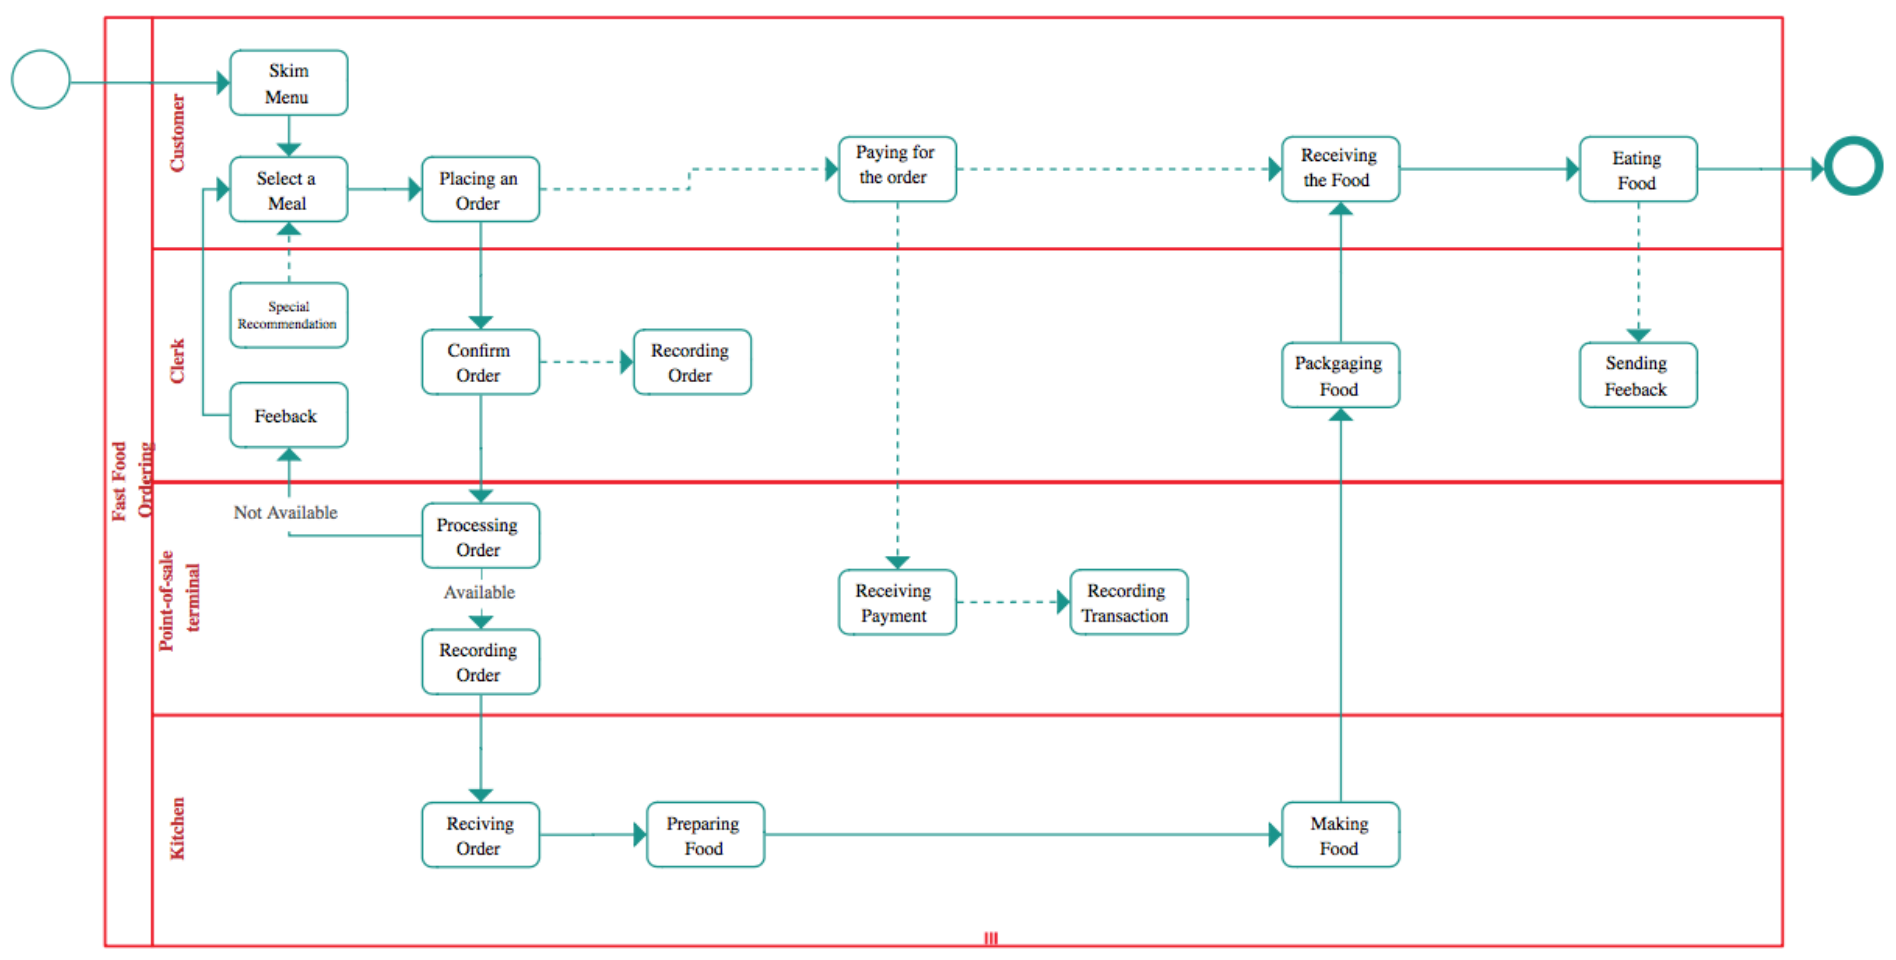
\includegraphics[width=0.9\textwidth]{./assets/t1/customer_figure.png}
  \caption{Customer-drawing workflow}
\end{figure}

Besides the previous requirement there are customized requests that have been made by the owners of the restaurant
These will be taken into consideration and implemented into the software:

\begin{itemize}
  \item The Customers should be able to interact with the Clerks without direct contact.
  \item Without having to install apps, there should be QR code and some other Web features for the customers.
  \item Customers can access this software on most platforms like mobile devices, tablets, laptops or even personal computers.
  \item The flexibility should be considered for multiple restaurants can be used if there is an expansion of quantity.
  \item The transaction rate measured recently is approximately 300 orders/day.
\end{itemize}

The eye-catching features that defines the software quality is the graphic design, which is also provided by the client
This software User Interface (UI) will mainly be based on these Figures below if there are no changes in the future:

\begin{figure}[H]
  \centering
  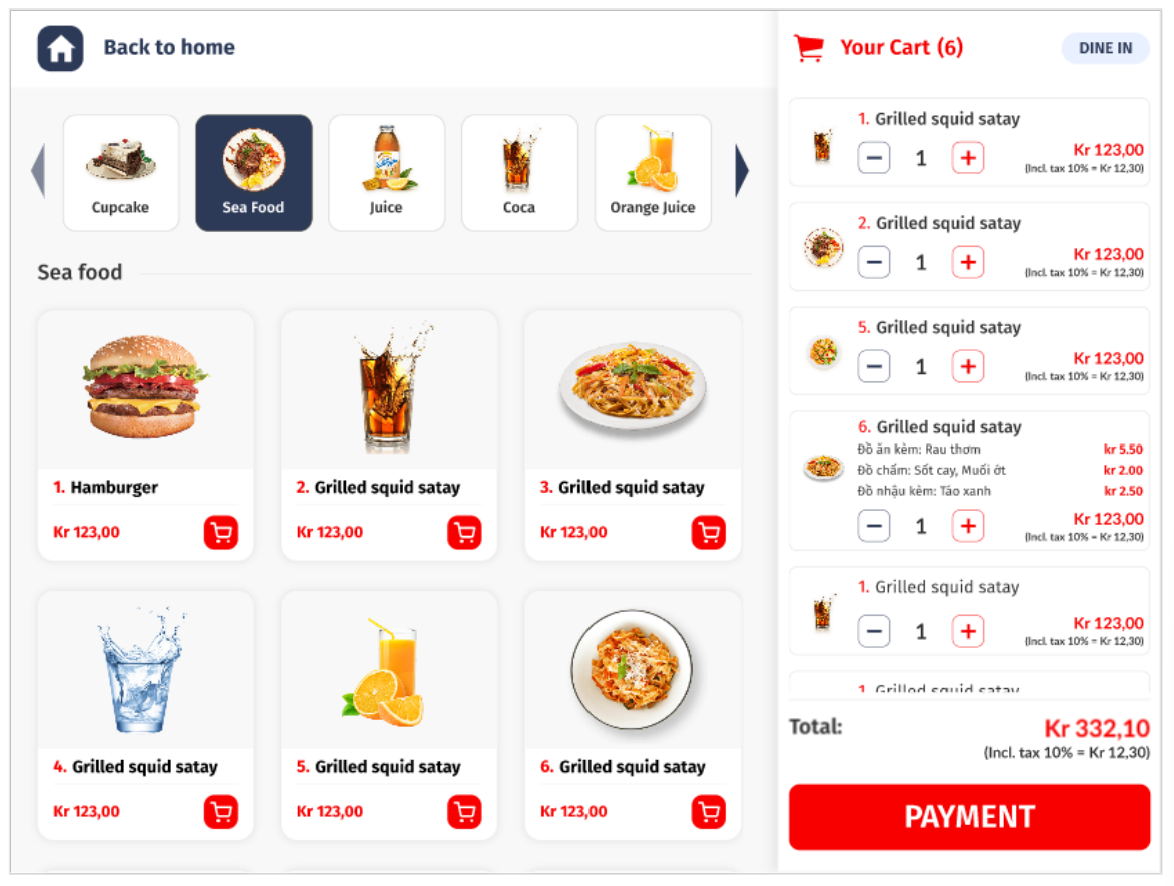
\includegraphics[width=\textwidth]{./assets/t1/UI_menu.png}
  \caption{The menu screen}
\end{figure}

This is the main menu for both take-away and dine-in customers.

\begin{figure}[H]
  \centering
  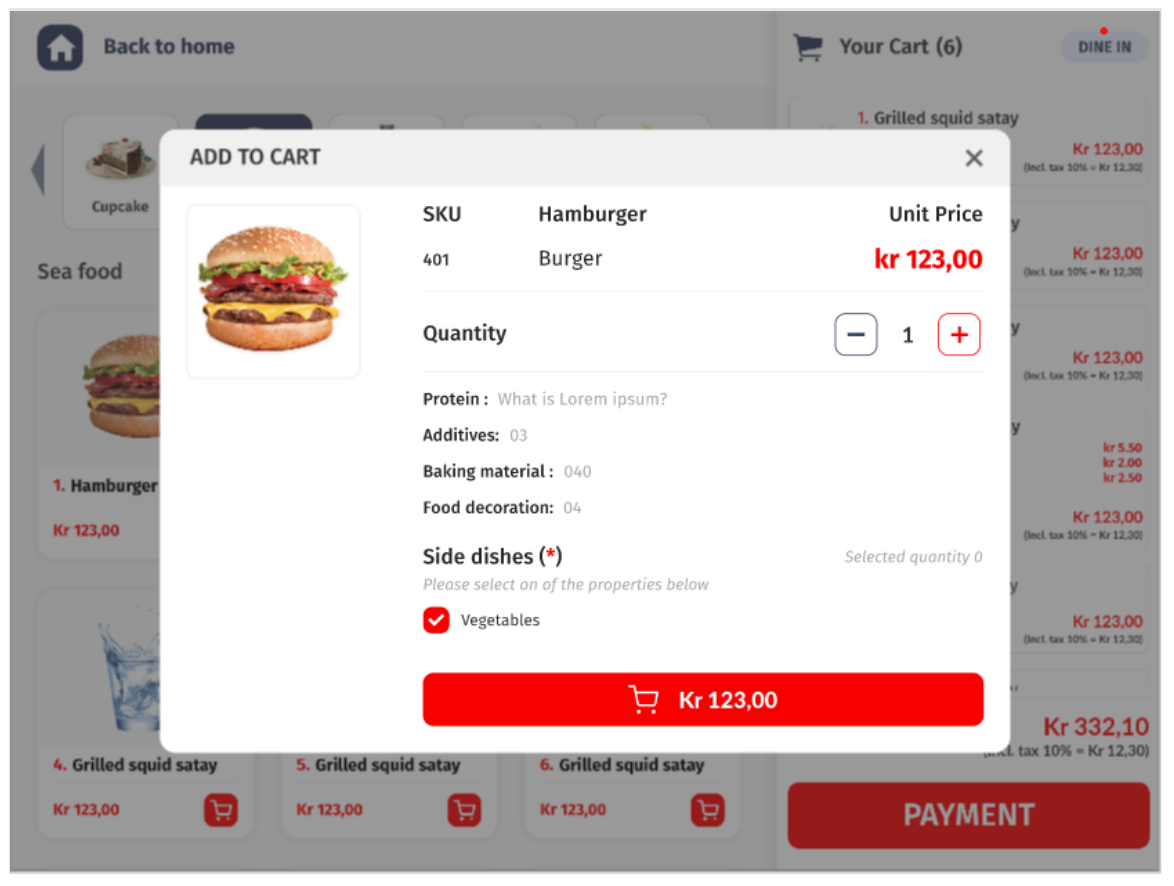
\includegraphics[width=0.9\textwidth]{./assets/t1/UI_detail.png}
  \caption{The detail item screen}
\end{figure}

This is the detail item screen when clicking to select an item in Figure 2
When changing the Quantity or click on the shopping button, returning to the Menu screen and update the sum-up Your Cart in the right hand side.

\begin{figure}[H]
  \centering
  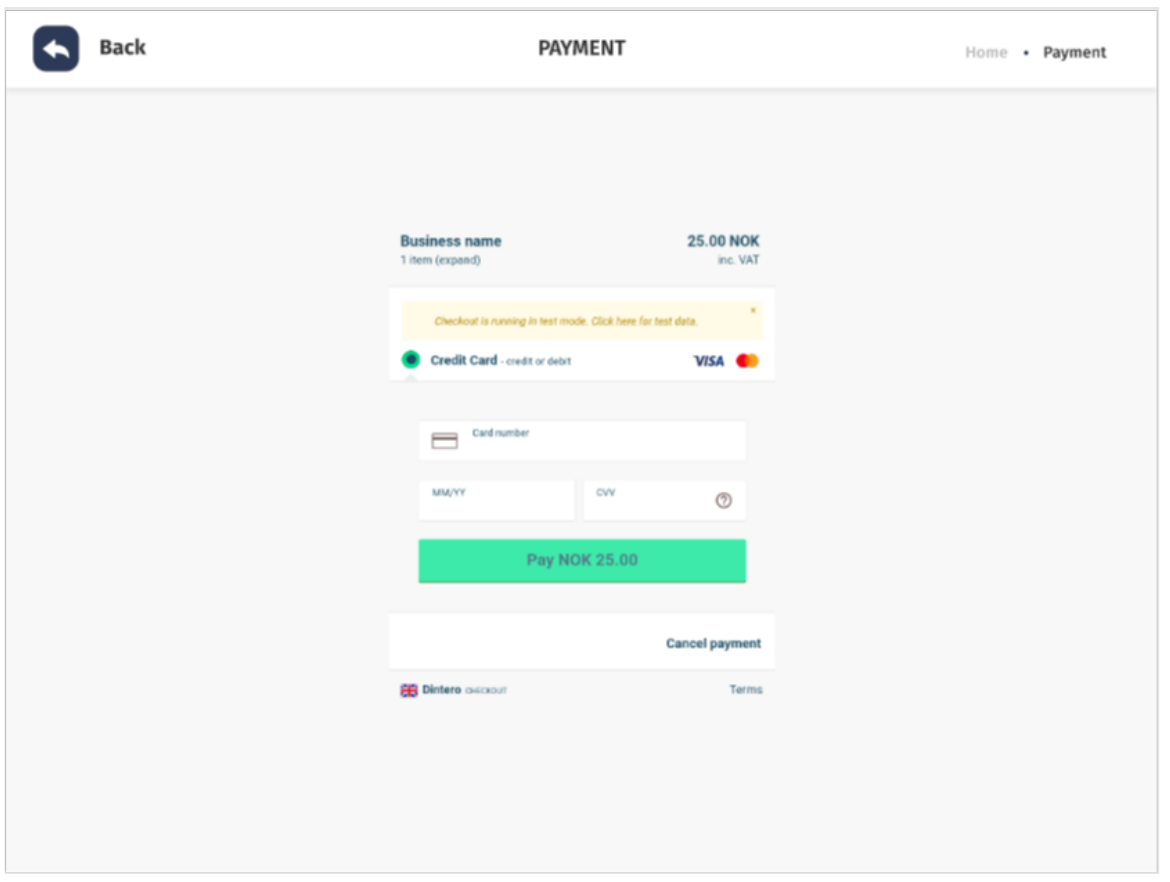
\includegraphics[width=0.9\textwidth]{./assets/t1/UI_payment.png}
  \caption{The payment page}
\end{figure}

\subsection{Scope} % TODO Wrong
Specifically, the system provides an automated price list and allows creation and printing of receipts based upon transactions of clients.
The system also enables creation and automatic updates of inventory whenever new entries or deletion of entries are made.
Only the management has access on the database for security reasons.
User accounts will be created to handle the daily transactions of the business, like payments and inventory.
Only those with such accounts can be able to access the system.
Also, the system will handle credit card transactions, support take-away options and also minimize work efforts across many work phases.

After hitting payment in Figure 2 will take the customer to this page for choosing the payment method or inserting credit card information.

\newpage

\section{Requirements}
\subsection{Functional Requirement}
The system should not allow direct contact between Clerks and Customers so there are separable interfaces for each actors.
\begin{enumerate}
  \item{Customers}
  \begin{figure}[H]
    \centering
    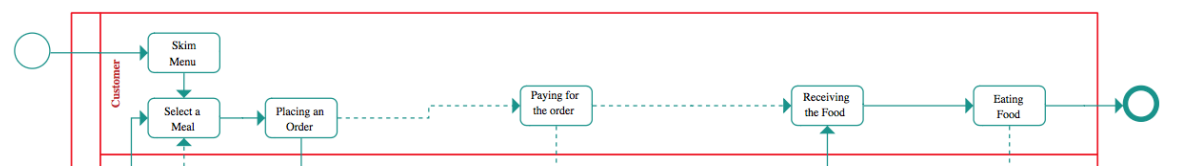
\includegraphics[width=0.9\textwidth]{./assets/t1/Customer_flow.png}
    \caption{The customer flow}
  \end{figure}
  \item[]According to the workflow, we can identify some functional requirements that meet the demand of the customers.
  \begin{itemize}
    \item Customers can order food on the menu.
    \item Customers can pay their bill.
    \item Customers can give special requirements for their order which can be seen by the cook.
    \item Customers can give feedback.
    \item Customers can view their transaction history.
  \end{itemize}
  \item{Clerks}
  \begin{figure}[H]
    \centering
    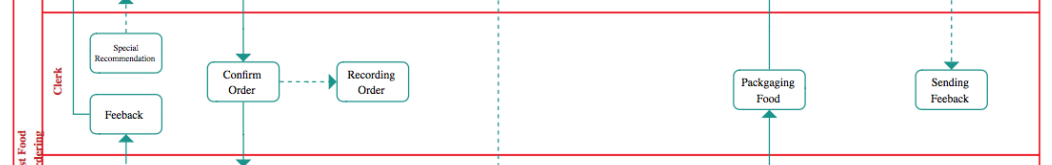
\includegraphics[width=0.9\textwidth]{./assets/t1/Clerk_workflow.png}
    \caption{The clerk workflow}
  \end{figure}
  \item[]Based on the workflow of the clerks, we can define some functional requirements for the system.
  \begin{itemize}
    \item The manager can customize their QR code.
    \item The clerks can give special recommendations to the customers.
  \end{itemize}
\end{enumerate}

\subsection{Non-functional Requirement}
According to the expectation of the restaurant owner about the system, we can define the non-functional requirements.
\begin{itemize}
  \item The system can be extendable in be use in multiple restaurants.
  \item The system should be usable from a mobile device, a laptop or a tablet device.
  \item The system should be implemented on the web.
  \item Customers can get access to the website via the QR code.
  \item The system should allow non-direct contact between Clerks and Customers.
\end{itemize}

\subsection{Full system use-case diagram}
From the workflow chart and the other party's requirements, we obtain the following use-case diagram.

\begin{figure}[H]
  \centering
  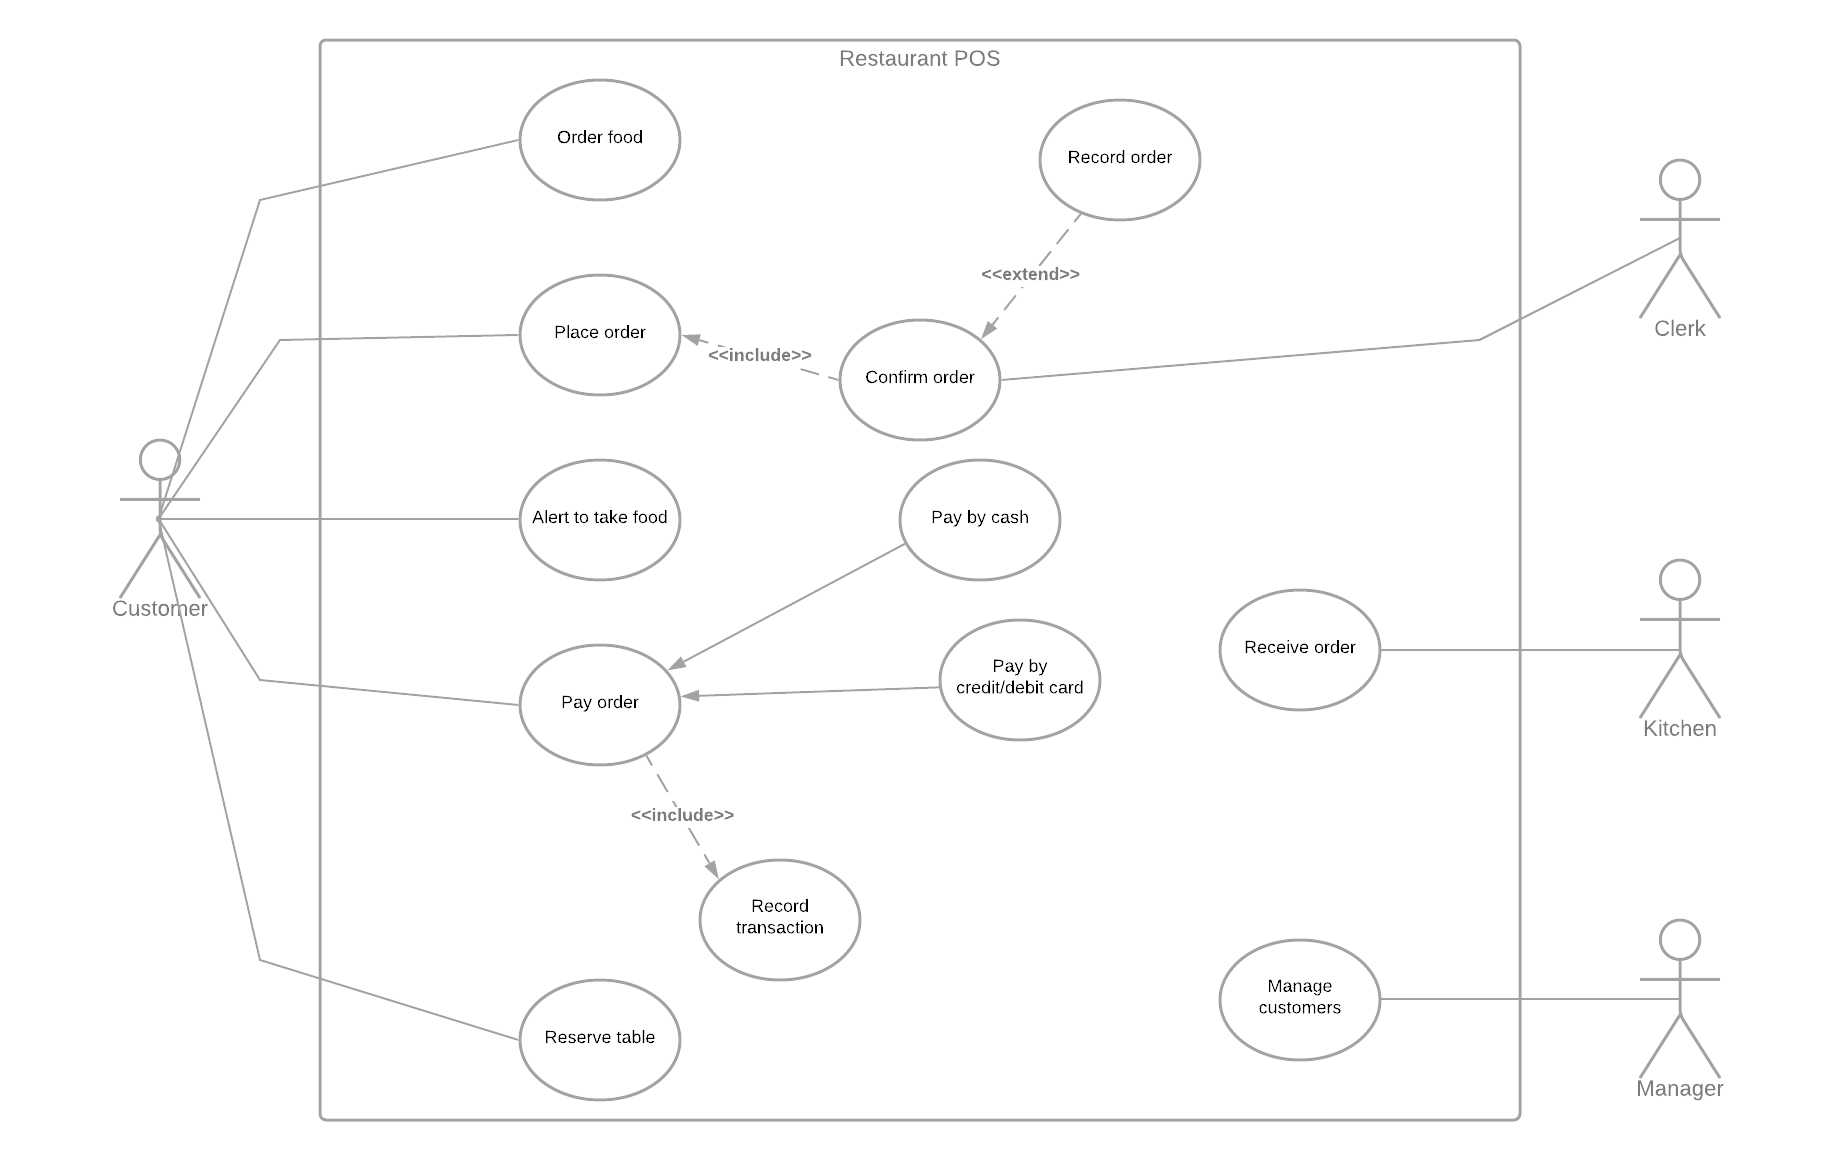
\includegraphics[width=0.9\textwidth]{./assets/t1/PieceOfSale.png}
  \caption{Full system use-case diagram}
\end{figure}

\newpage

\section{Diagram and table for pay order use-case}
The following use-case diagram and table are for the pay order use-case.

\begin{figure}[H]
  \centering
  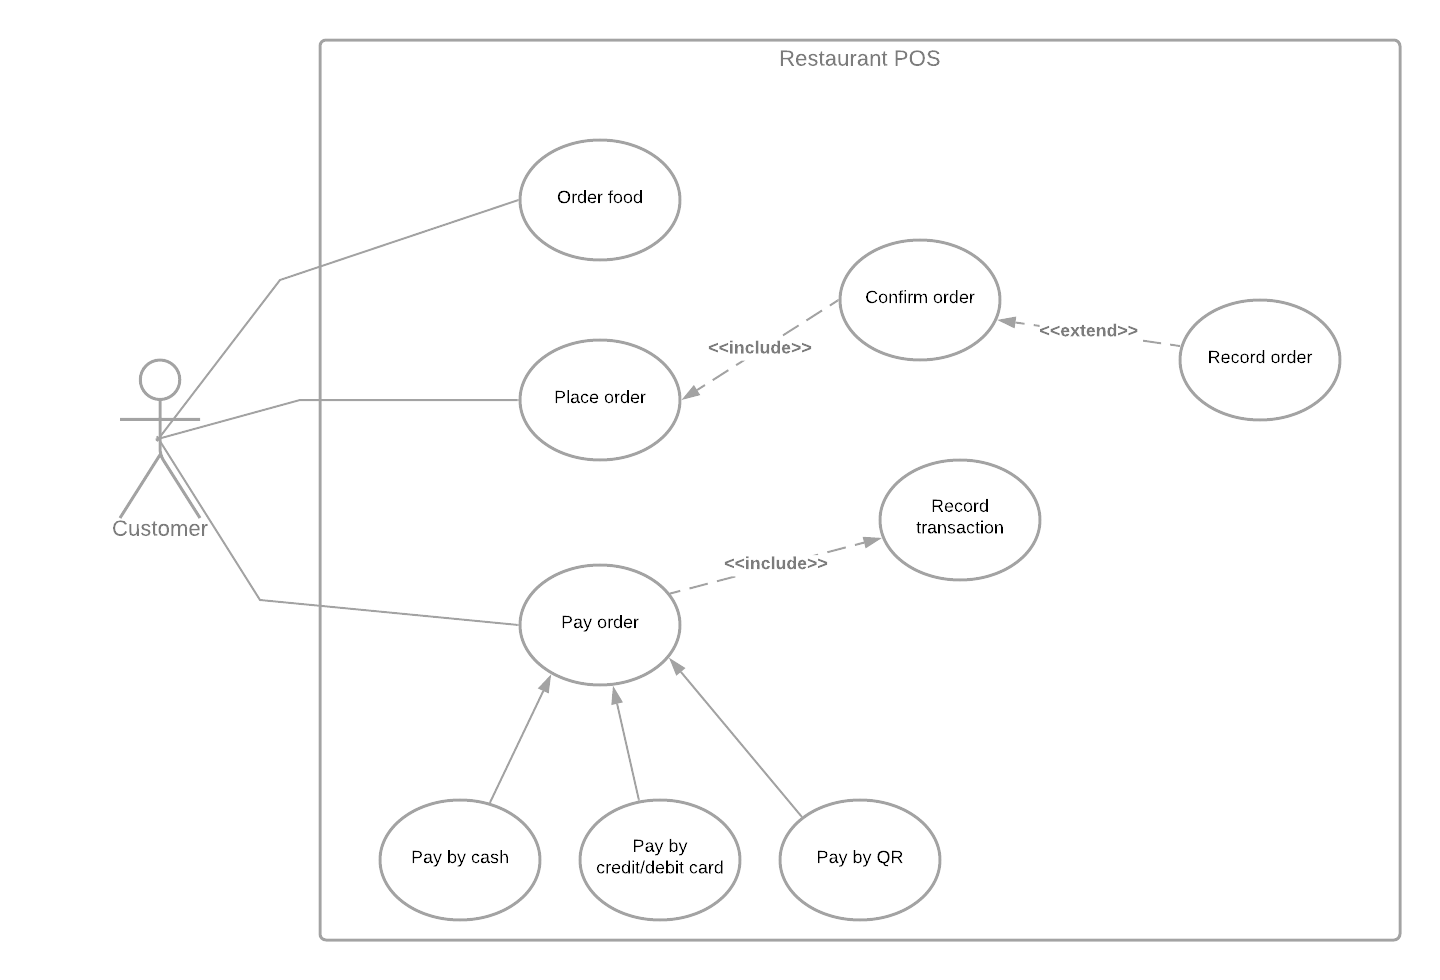
\includegraphics[width=0.9\textwidth]{./assets/t1/PayOrder.png}
  \caption{Pay order use-case diagram}
\end{figure}

\begin{center}
  \begin{tabular}{*{2}{l}}
    \toprule
    Use-case name & Pay order / Pay the bill                                    \\
    Actors        & Customer                                                    \\
    Pre-condition & An order is confirmed                                       \\
    Trigger       & Customer wants to pay the bill                              \\
    Basic path    & 1. POS displays bill to customer                            \\
                  & 2. Customer chooses a payment method                        \\
                  & 3. Customer pays using the chosen method                    \\
                  & 4. POS confirms and saves the transaction record or receipt \\
    \bottomrule
  \end{tabular}
\end{center}
